\documentclass[a4paper,12pt,twoside,openright]{report}

% information defines
\def\authorname{Oliver D.\ N.\ Hope\xspace}
\def\authorcollege{Jesus College\xspace}
\def\authoremail{oliver.hope@cst.cam.ac.uk}
\def\dissertationtitle{Reinforcement learning techniques for generalisable data-driven routing}
\def\wordcount{Hopefully around 12000}


%\usepackage[dvips]{epsfig,graphics} 
\usepackage{epsfig,graphicx,verbatim,parskip,tabularx,setspace,xspace}
\usepackage{fontspec}
\usepackage[backend=biber]{biblatex}
\defaultfontfeatures{Ligatures=TeX}
\setmainfont{Linux Libertine O}
\usepackage{amsmath}
\usepackage{bm}
\usepackage{algorithm}
\usepackage{algcompatible}
\usepackage{algpseudocode}

% remove this when done
\usepackage{todonotes}

% fix comment alignment in algorithm blocks
\renewcommand{\Comment}[2][.525\linewidth]{%
  \leavevmode\hfill\makebox[#1][l]{$\triangleright$~#2}}
  
% perform detailed wordcount, TODO: remove when done
\usepackage{shellesc}
\newcommand{\detailtexcount}[1]{%
  \ShellEscape{texcount -merge -sum -q #1.tex output.bbl > #1.wcdetail }%
  \verbatiminput{#1.wcdetail}%
}

\addbibresource{refs.bib}

%% START OF DOCUMENT
\begin{document}

\detailtexcount{main}

%% FRONTMATTER (TITLE PAGE, DECLARATION, ABSTRACT, ETC) 
\pagestyle{empty}
\singlespacing
% title page information
\begin{titlepage} 

\begin{center}
\noindent
\huge
\dissertationtitle \\
\vspace*{\stretch{1}}
\end{center}

\begin{center}
\noindent
\huge
\authorname \\
\Large
\authorcollege      \\[24pt]
%\begin{figure}

\includegraphics{figures/CUni3.pdf}
%\end{figure}
\end{center}

\vspace{24pt} 

\begin{center}
\noindent
\large
{\it A dissertation submitted to the University of Cambridge \\ 
in partial fulfilment of the requirements for the degree of \\ 
Master of Engineering in Computer Science} 
\vspace*{\stretch{1}}
\end{center}

\begin{center}
\noindent
University of Cambridge \\
Department of Computer Science and Technology \\
Computer Laboratory     \\
William Gates Building  \\
15 JJ Thomson Avenue    \\
Cambridge CB3 0FD       \\
{\sc United Kingdom}    \\
\end{center}

\begin{center}
\noindent
Email: \authoremail \\
\end{center}

\begin{center}
\noindent
\today
\end{center}

\end{titlepage} 

\newpage
\vspace*{\fill}

\onehalfspacing
\newpage
{\Huge Declaration}

\vspace{24pt} 

I, \authorname of \authorcollege, being a candidate for Computer Science Tripos, Part III, hereby declare that this report and the work described in it are my own work, unaided except as may be specified below, and that the report does not contain material that has already been used to any substantial extent for a comparable purpose.

\vspace{24pt}
Total word count: \texcount{main}

\vspace{60pt}
{\large Signed}: $
\begin{array}{l}
\includegraphics[width=7em]{figures/signature.pdf}
\end{array}
$

\vspace{12pt}
{\large Date}: \today


\vfill

This dissertation is copyright \copyright 2020 \authorname. 
\\
All trademarks used in this dissertation are hereby acknowledged.



\newpage
\vspace*{\fill}

\singlespacing
\newpage
{\Huge \bf Abstract}
\vspace{24pt} 

This project seeks to apply deep reinforcement learning (RL) techniques with graph neural networks to the space of intradomain traffic engineering in order to minimise link congestion. Recently, there has been work in this space from Valadarsky et al. in the paper ``Learning to route with Deep RL'' where the authors achieved some success using RL with a multilayer perceptron (MLP) policy architecture. However, this approach suffers from a level of rigidity in that it cannot easily generalise to new networks or traffic types.

Aside from this work, there has been an explosion of research into graph neural networks (GNNs) which are a class of neural network the operates specifically on the structure of graphs. These make it easier to create only the intended relational inductive biases in policy design and have had much success in many fields, especially in terms of generalising solutions across different graphs.

In this project, we aim to combine these two ideas: the routing methods from Valadarsky et al. with GNNs to allow for generalisation. We provide a new environment in which different strategies can be implemented and tested, including different types of policy, traffic, and utility function. We also present the design of GNN-based policies that seek to solve this problem. Finally, we provide a comprehensive assessment of the different techniques, with a particular focus on their capability to generalise to different traffic patterns and network topologies.

\newpage
\vspace*{\fill}


\pagenumbering{roman}
\setcounter{page}{0}
\pagestyle{plain}
\tableofcontents
\listoffigures
\listoftables

\onehalfspacing

%% START OF MAIN TEXT 
\chapter{Introduction}

% this has to be done after the chapter start so can't put in top level :'(
\pagenumbering{arabic}
\setcounter{page}{1}

Routing has always been an integral part of the functioning of the internet as it is required for data to traverse a network from source to destination successfully. Historically, strategies have mainly focussed on those that can be calculated in a distributed manner, are functionally correct, and are robust to network changes all while providing reasonable performance (both in the time to calculate routes and their effect on the traffic itself). More recently, and especially with the advent of \ac{sdn}, there has been a concerted effort to exert more control over how traffic is routed. This control has either been used to implement policies that favour types of traffic, particular customers, or simply aim to achieve particular notions of performance on the network.

In the area of intradomain routing where this kind of control is possible, one particular focus has been on minimising link over-utilisation, as congestion can have significant impacts on network performance for the end-user. To minimise congestion successfully, such protocols must take into account how one traffic flow on the network impacts the other traffic flows, which leads us to data-driven routing. It is already known how to route optimally given a set of traffic demands over a network. However, in general, these demands cannot be known in advance. Therefore, there have been efforts to create routing schemes that will generally give good congestion performance no matter the particular traffic demands on the network (called oblivious routing). Further research has aimed to make these routing strategies include some notion of the current traffic.

A recent paper: "Learning To Route with Deep RL" examined whether we can use reinforcement learning to produce better routing strategies than the oblivious approach. It worked under the assumption that there is some regularity in sequences of traffic demands on a network and that using this regularity we can get closer to the optimal performance. This work produced some impressive results. However, once it has learnt to route on a particular network, due to the rigid structure of the neural network used to make the policy, this cannot be applied to a different network. This issue may seem relatively small, that is until one takes into account the fact that networks often change, often due to temporary outages. If, for example, a link or node in the network were to be temporarily off-line, then such a system would be unable to provide a routing scheme.

This project seeks to take the problem specified in ``Learning to Route with Deep RL'' as well as its solution and extend its domain to cover changing the structure of the network itself. In other words, the aim is to use \ac{rl} to enable the creation of close-to-optimal routings for a network, given a history of traffic demands on that network, and that this should be able to generalise both over different demand sequences for the same network and different demand sequences for entirely different networks. Graph generalisation is a useful goal as it allows a learned routing strategy to continue to work on networks suffering faults such as dropped links and also may mean that the model would not need to be retrained to be used on different networks. Finally, we aim to show that this is not just a toy problem and solution but leads to results on real-world datasets.

In summary, this study makes the following research contributions:
\begin{itemize}
  \item Provides an environment for experimenting with \ac{rl} in data-driven routing
  \item Designs a new mapping from edge weights to a fully specified multipath routing
  \item Introduces policy designs for approaching data-driven routing in a way that is generalisable to different network topologies
  \item Presents a comprehensive assessment of the performance of different techniques with a specific focus on generalisability over traffic patterns and network topologies.
\end{itemize}

The rest of the dissertation is structured as follows: chapter~\ref{chapter:background} introduces both previous research in this area and the research on which we base techniques in this work; chapter~\ref{chapter:problem} presents the formal specification of the problem, how we designed the environment, and techniques that made the problem and routing feasible to be performed using \ac{rl}; chapter~\ref{chapter:learning} describes how the \ac{rl} policy was designed and trained, and the structure of the \acp{gnn} used; chapter~\ref{chapter:evaluation} explains the evaluation framework and examines the results of the experiments performed; and chapter~\ref{chapter:conclusions} summaries the findings and contributions of the entire work as well as providing an insight into possible future work.


\chapter{Background and related work}
\label{chapter:background}

In this chapter I provide an overview and summary of the research that has been used by and influenced this work as well as covering similar research that has been performed. This includes a look at traffic engineering, reinforcement learning techniques, the advent of graph neural networks and other approaches to optimising networking using reinforcement learning.


\section{Traffic engineering}

\subsection{Intradomain routing}

The field of internet traffic engineering contains the problem of how to control and manage computer networks. One such problem is that of intradomain routing. Intradomain routing focusses on what paths data should take on a single network entirely controlled by one entity who generally has complete knowledge of the contents of the network and control over how the routing is to be managed (e.g. which protocol to use). An example of what we mean by a network controlled by one entity in this context is an autonomous system (AS). Autonomous systems can scale from the size of a small company to that of a large internet service provider (ISP).

The benefit of working inside and AS rather than the full internet is the complete knowledge and control which gives a lot more scope for achieving optimality concerning network control. For example, a network administrator can decide what their priorities are for the network and internally apply policy and routing that reflects those aims. Common aims are minimising latency between source and destination or minimising link utilisation to avoid congestion and packet loss. Examples of the most common protocols used for intradomain routing are RIP\cite{rfc2080} and OSPF\cite{rfc5340} which both minimise distance which generally equates to latency.

\subsection{Data-driven routing}

In the previous section intradomain routing was introduced along with the protocols commonly used for routing. These protocols have generally led to good performance and are deployed almost everywhere. However, they only take into account the structure of the network itself and not the traffic that goes over it. As different flows on the network can interfere with each other the data on the network can have an impact on the utility of the routing used. Therefore, if possible, taking into account the traffic conditions when performing routing can have a significant positive impact on performance (whether this be measured by latency, throughput or some other metric). This leads us to data-driven routing.

Data-driven routing seeks to make routing decisions that take into account the impact of traffic on the network. This is often to provide improved performance by reducing link congestion which is the utility which will be focussed on here.

\subsection{Multicommodity flow}
\label{section:multicommodity}

The problem of data-driven routing can in fact be modelled as a multicommodity flow problem. The multicommodity flow problem is simply a network flow problem with multiple demands between different source and sink nodes. It consists of a flow network $G(V,E)$ where each edge $(u,v) \in E$ has a capacity $c(u,v)$. Then we wish to place commodities $K_i = (s_i, t_i, d_i)$ on the network where $s_i$ is the source, $t_i$ is the sink and $d_i$ is the demand (the amount of data to pass between source and sink). Finally the following constraints must be satisfied:

\begin{enumerate}
    \item Flow on a link must not exceed its capacity:\\
    $\forall (u,v)\in E:\,\sum_{i=1}^{k} f_i(u,v)\cdot d_i \leq c(u,v)$
    \item Flow entering and exiting a node must be conserved:\\
    $\sum_{w \in V} f_i(u,w) - \sum_{w \in V} f_i(w,u) = 0 \quad \mathrm{when} \quad u \neq s_i, t_i$
    \item The entire flow of a commodity must exit its source:\\
    $\sum_{w \in V} f_i(s_i,w) - \sum_{w \in V} f_i(w,s_i) = 1$
    \item The entire flow of a commodity must be absorbed at the sink:\\
    $\sum_{w \in V} f_i(w,t_i) - \sum_{w \in V} f_i(t_i,w) = 1$
\end{enumerate}

In this framework we are able to specify any valid routing we wish (including splitting one flow across multiple routes) but importantly we can also optimise the routing under a given utility function using linear programming in polynomial time for a specified set of commodities (as long as we allow fractional flows)\cite{cormen2009introduction}. This in effect means optimal data-driven routing for reducing link congestion is solved except for the important fact that in most cases we do not know the traffic demands on a network in advance so the routing would always lag the commodities it was optimised for.

\subsection{Current approaches to reducing link congestion}

Current approaches to traffic engineering often rely on the use of software defined networking (SDN) which separates the control plane and data plane and allows for more complicated and custom routing schemes to be easily deployed\cite{doi:10.1002/sec.1737}. On top of these SDN systems many different methods have been used to achieve better network performance in the face of high traffic demands.

One such method are forms of oblivious routing\cite{Bansal2008} which seeks to reduce congestion on links in a network without the knowledge of what the traffic demands are. Early examples of approaches are that of R\"acke\cite{racke2002minimizing} who showed that it is possible to have an optimal oblivious routing and Azar\cite{azar2004optimal} who proved that this can be calculated in polynomial time. Since then, small, incremental improvements have been made, improving calculation time or allowing for different utility functions to be specified\cite{kodialam2008advances}.

However, it is still possible to do better than oblivious routing if you have some knowledge of the traffic. One seminal work in this area is SMORE\cite{kumar2018semi} which combines oblivious routing and adaptive sending rates to improve reliable network performance under all kinds of operating conditions.

On will notice that while all of these methods do successfully improve network performance in the sense of reducing link congestion, they are all fundamentally limited by their knowledge (or lack thereof) of the current operating conditions of the network they are creating a routing strategy for. 


\section{Machine learning}

\subsection{Reinforcement learning}

Reinforcement learning (RL)\cite{sutton2018reinforcement} is a subsection of machine learning the third of the three paradigms, the other being supervised and unsupervised learning. It is concerned with training agents to take actions in some specified environment and achieve a goal in that environment as can be seen in Figure~\ref{fig:reinforcement_learning}. Commonly the agent makes choices using a neural network which is trained using any one of multiple algorithms designed for this purpose (all with different trade-offs). RL is powerful as it does not require an analytical model of the environment being used as it is able to find out how to act through exploration alone. RL has been used successfully in many fields approaching many different problems such as in robotics\cite{}, game-playing\cite{}, \todo{fill in these citations} and general optimisation with one recent success being playing board games to a super-human level with AlphaZero\cite{Silver1140}.

\begin{figure}
    \centering
    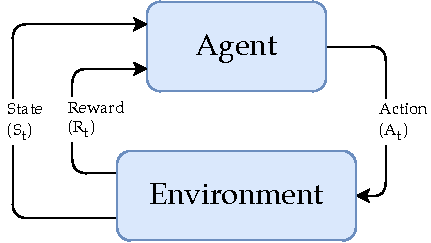
\includegraphics[width=0.5\textwidth]{figures/reinforcement_learning.pdf}
    \caption{The structure of a reinforcement learning problem: the interaction of agent and environment}
    \label{fig:reinforcement_learning}
\end{figure}

Formally, a RL problem is generally framed with the environment modelled as a finite Markov decision process (MDP) which can be defined as the 4-tuple $(S, A, P_a, R_a)$ where:
\begin{itemize}
    \item $S$ is a finite set of states
    \item $A$ is a finite set of actions
    \item $P_a(s,s')$ is the probability that action $a$ in state $s$ at time $t$ will lead to state $s'$ at time $t + 1$
    \item $R_a$ is the reward received after transitioning from state $s$ to state $s'$, due to taking action $a$
\end{itemize}

With a MDP defined as our environment it is then necessary to create an agent to interact with it. Generally such an agent is implemented by a policy which will return an action given an observation (which is a set of features probabilistically derived from the current state of the environment). This policy can take many forms but in deep RL as used in this research it takes the form of a neural network.

The final piece of the RL puzzle is a way to make the policy act how we want it to (or formally to maximise the reward it can achieve in an episode). Again, there are multiple ways to do this. One such method is the policy gradient method with the first prominent example being REINFORCE\cite{williams1992simple}. One branch of this to have gained traction in particular are actor-critic algorithms. These have two main parts:

\begin{itemize}
    \item The \emph{critic} which updates the value function ($V(s)$, the expected reward from a given state) given feedback from the environment.
    \item The \emph{actor} which updates the policy ($\pi(a|s)$, the probability of choosing an action in a state) using feedback from the critic.
\end{itemize}

PPO\cite{schulman2017proximal} is an example of an actor-critic algorithm that achieves good sample efficiency and performance while maintaining a fairly simple implementation (relative to similar algorithms). This is mainly because of how it restricts the maximum size of policy updates. It has had notable successes such as beating world champions in a live game of Dota 2\cite{openai2019dota}.

\subsection{Graph neural networks}

Graph neural networks (GNNs)\cite{gori2005new,scarselli2008graph} are a form of neural network that has gained considerable 
traction over the last few years. This is because, in the same way that convolutional neural networks (CNNs) have been used with much success on images as pixels form a grid and are often related to their neighbouring pixel, many other datasets are graph structured with relations to neighbouring nodes being an important part of this structure. GNNs effectively allow us to generalise the CNN model onto graphs. \todo{give some example uses} There are many different types of GNN with different trade-offs as described in countless surveys of the subject\cite{zhou2018graph,Wu_2020}.

Possibly the most general model, allowing for restrictions to define the different subtypes of graph network is that proposed by Battaglia et al.\cite{battaglia2018relational}. They propose that combinatorial generalisation is crucial to learning and that this relies on the integration of structured and unstructured approaches. All networks contain some level of structure leading to relational inductive biases but it is only graph networks that give fine-grained control over these biases to fully harness the structure present in the problem being solved and without implying structure that is not present.

The model presented by Battaglia et al.\ defines a Graph Network (GN) Block which takes as input a graph and returns a graph. Here a graph is defined to be the 3-tuple $G = (\bm{u}, V, E)$ where $\bm{u}$ is a global attribute vector, $V = \{\bm{v}_i\}_{i=1:N^v}$ is the set of vertex attribute vectors, and $E = \{(\bm{e}_k, r_k, s_k)\}_k=1:N^e$ is the set of edge attribute vectors and their source and destination vertices.

The graph block itself computes over an input graph as shown in Algorithm~\ref{algorithm:graph_block}. This algorithm contains three $\phi$ functions which update attribute information and three $\rho$ functions which pool attribute information to be used in the updates. It is the coefficients in these functions that are learn and the ability to change the operations that these functions perform that allows for the flexibility to implement many different types of GNN.\todo{insert Graph Network Block Diagram maybe?}

\begin{algorithm}[t]
\small
\begin{algorithmic}
\Function{GraphNetwork}{$E$, $V$, $\mathbf{u}$}
    \For {$k\in \{1\ldots{}N^e\}$}
        \State $\mathbf{e}_k^\prime\gets \phi^e\left(\mathbf{e}_k, \mathbf{v}_{r_k}, \mathbf{v}_{s_k}, \mathbf{u} \right)$
        \Comment{1. Compute updated edge attributes}
    \EndFor
    \For {$i\in \{1\ldots{}N^n\}$}
        \State \textbf{let} $E'_i = \left\{\left(\mathbf{e}'_k, r_k, s_k \right)\right\}_{r_k=i,\; k=1:N^e}$
        \State $\mathbf{\bar{e}}'_i \gets \rho^{e \rightarrow v}\left(E'_i\right)$
        \Comment{2. Aggregate edge attributes per node}
        \State $\mathbf{v}'_i \gets \phi^v\left(\mathbf{\bar{e}}'_i, \mathbf{v}_i, \mathbf{u}\right)$
        \Comment{3. Compute updated node attributes}
    \EndFor
    \State \textbf{let} $V' = \left\{\mathbf{v}'\right\}_{i=1:N^v}$
    \State \textbf{let} $E' = \left\{\left(\mathbf{e}'_k, r_k, s_k \right)\right\}_{k=1:N^e}$
    \State $\mathbf{\bar{e}}' \gets \rho^{e \rightarrow u}\left(E'\right)$
    \Comment{4. Aggregate edge attributes globally}
    \State $\mathbf{\bar{v}}' \gets \rho^{v \rightarrow u}\left(V'\right)$
    \Comment{5. Aggregate node attributes globally}
    \State $\mathbf{u}' \gets \phi^u\left(\mathbf{\bar{e}}', \mathbf{\bar{v}}', \mathbf{u}\right)$
    \Comment{6. Compute updated global attribute}
    \State \Return $(E', V', \mathbf{u}')$
\EndFunction
\end{algorithmic}
\caption{Steps of computation in a full GN block. (Taken from \cite{battaglia2018relational})}
\label{algorithm:graph_block}
\end{algorithm}


\section{Approaches to routing using reinforcement learning techniques}

There have thus far been multiple approaches to network-related problems using machine learning and especially reinforcement learning techniques. There is a growing body of work covering areas from routing to deep packet inspection. Specifically in the area of routing, there has been reinforcement research for quite a while with an early seminal paper introducing the idea of Q-routing in 1994\cite{boyan1994packet} which attempts to use distributed on-device agents to route packets so as to minimise delay. Many pieces of work have followed a similar vein gradually improving on Q-routing with ever more complex policies\cite{you2019toward,Ali2019HierarchicalDD}.

A separate issue is the traffic engineering problem where one can make global decisions for a large scale network (such as an autonomous system) on a longer timescale. In this area there has recently been one major work: ``Learning to Route with Deep RL''\cite{valadarsky2017learning} which is the paper who's research our work seeks to extend and improve. The paper introduces the problem of knowing the history of traffic demands for a given network and using it along with a neural network to predict what routing should be used on the network in the next timestep to minimise link over utilisation. This is performed using reinforcement learning with a novel translation from action to routing.

Similarly, another paper: ``A Deep-Reinforcement Learning Approach for Software-Defined Networking Routing Optimisation''\cite{stampa2017deep} sought to use reinforcement learning to find good routes for a given traffic matrix. However, this means that the matrix must be known in advance and we already have deterministic algorithms than can find optimal routings given a traffic matrix. Also, within the last few months there has been some other work on optimising routing, this time looking at link utilisation and using GNNs\cite{Sawada2020NetworkRO}. However, it learns to cope with the current traffic flow as it is occurring and is distributed rather than centralised.


\chapter{Problem specification and approaches}
\label{chapter:problem}

\section{Introduction}
In this chapter we describe the formal specification of the problem to be solved whilst also introducing some tactics that have been used to make this more feasible. This includes a description of methods to reduce the action space and how this can still result in a fully defined routing. As part of this we introduce an algorithm to remove unwanted cycles from a network graph.

\section{Data-driven routing}
\label{section:routing}
In the introduction it was described that this project seeks to perform more optimal routing in the presence of knowledge of traffic demands than oblivious techniques. To do this we must first define the routing model it acts on. We take a similar model to that of Valadarsky\cite{valadarsky2017learning}. In this context we consider a static network upon which we can specify a routing, and which also has a set of traffic demands associated with it in the form of traffic matrices. Formally we have:
\begin{itemize}
  \item The \emph{network} which is modelled as a directed graph where all the edges have a link capacity: $G=(V,E,c)$ where $V$ is the set of vertices, $E$ is the set of edges and $c : E \rightarrow \mathbb{R}^+$ is a function mapping each edge in the graph to its capacity.
  \item The \emph{routing} which for each flow (demand and source and destination pair) specifies at each vertex how much of that flow should be sent down each of its edges to each of its neighbours. Therefore, if we define $\Gamma(v)$ to be the set of all neighbours of vertex $v$ then we can define a routing to be $\mathcal{R}_{v,(s,t)} : \Gamma(v) \rightarrow [0,1]$ with $\mathcal{R}_{v,(s,t)}(u)$ as the proportion of the flow passing from $s$ to $t$ through vertex $v$ that is forwarded to vertex $u$. Importantly, any routing specified must obey the two constraints:
    \begin{enumerate}
      \item No traffic is lost between source and destination:\\
        $\sum_{u \in \Gamma(v)}{\mathcal{R}_{v,(s,t)}(u)} = 1 \qquad \forall s, t \in V \wedge v \neq t$
      \item All traffic for a destination is absorbed at that destination:\\
        $\sum_{u \in \Gamma(v)}{\mathcal{R}_{t,(s,t)}(u)} = 0 \qquad \forall s, t \in V$
    \end{enumerate}
  \item The \emph{demands} which can be represented as an $D \in \mathbb{R}^{|V|\times|V|}$ matrix called a demand matrix (DM) where each element $D_{st}$ is the traffic demand between the source $s$ and destination $t$.
\end{itemize}

With these definitions we can now fully describe the movement of traffic over a network. The rest of this work will use just this system and no more or less when talking about networks, routings or demands. In examples we will assume that the network itself is fixed and that traffic is described by sequences of DMs, each representing a discrete time step, which are also fixed. The only thing we are allowed to modify is the routing strategy. Given the above structure, we can define some notions of goodness of a particular routing. In particular, as our aim is to reduce congestion we will make our utility function that of minimising link over-utilisation.

This can be defined to be minimising $U_{max}$ in:\\
$\forall (u,v) \in E: U_{max} > U(u,v)$\\
where $U(u,v)$ is the utilisation of the link $(u,v)$.


\section{The environment}
So that it would be possible to both train and evaluate approaches to the defined problem, it was necessary first to construct an environment to simulate the desired responses that an RL agent could interact with. For easy interoperability with existing libraries, it was decided that this environment should have an OpenAI Gym\cite{brockman2016openai} API. Alongside the internal operations of the environment being correct, its interface to the RL agent is important as it has a large impact on how well the agent can learn. We will now proceed to discuss how the environment calculates rewards, the format of observations it gives to the agent and the format of actions it receives form the agent.

\subsection{Reward calculation}
As the optimal routing that can be achieved on a given graph varies for different demand matrices, the reward cannot simply be derived from the calculation of the maximum link utilisation. Fortunately, as described in section~\ref{section:multicommodity} we know that an optimal routing does exist and it can be found in polynomial time with linear programming. Therefore, the environment implements a linear solver for the optimal routing to calculate the optimal link utilisation\footnote{The solver is implemented on top of Google OR-Tools\cite{ortools}}. Then, the reward is derived by comparing the routing produced by the RL agent to the calculated optimal routing. This is presented in equation~\ref{equation:reward} where $U_{max}$ is the maximum link utilisation.
\todo{maybe also put the utility function definition here?}

\begin{equation}
  \label{equation:reward}
  \mathrm{reward} = -\frac{U_{max_{agent}}}{U_{max_{optimal}}}
\end{equation}

\subsection{Observations}
In the original ``Learning to route'' paper, an observation was a history of traffic demands, which was presented as a list of traffic matrices which was then flattened for input to the MLP. However, this works aims to make the solution generalisable over graphs of different shapes using GNNs. As GNNs work on graphs, it is possible to vary both the number of vertices and edges that are input to a GNN (something not possible with an MLP). However, this previous way of managing demands as observations would no longer work. The reason for this is that a sensible way to input the demands to the GNN would be to place the demands associated with each vertex on that vertex as vertex attributes. The issue here is that the number of demands a vertex has scales with the number of nodes in the graph. Therefore the size of node attributes in the GNN would have to grow as more vertices are added which is unfortunately not possible within the structure.

To solve this issue we had to find a way to associate the demands with the correct nodes in a way that would still allow the agent to learn but would require a constant amount of space per vertex as the graph grows. The solution used to this problem was summing for each vertex the total outgoing flow and incoming flow meaning that the observation size is now $O(|V|)$ as opposed to $O(|V|^2)$ and so can be used with a GNN.

One other important addition to make this new structure work was normalising the inputs as otherwise the more vertices in a graph, the higher the totals for each vertex will on average be which is unwanted behaviour.

\subsection{Action space}
Following on from the definitions given in section~\ref{section:routing}, we can see that one valid way for the agent to assign a routing would be to provide splitting ratios for each edge under each flow. However, this would require an output of $|V|\times(|V|-1)\times|E|$ separate values. Unfortunately, this size of action space is too big to learn successfully. If we make some approximating assumptions about the routing (which will no longer allow us to achieve the optimal routing but still allow us to get closer than oblivious strategies) then we can reduce this output size.

A first method to reduce the action space size is to ignore the source of any packets, forming a destination-only routing. This reduces the size to $|V|\times|E|$. However, this is still to large so instead we had to create a method of deriving routing strategies from setting weights of edges, creating an action space with only $|E|$ values. This was finally small enough to achieve good results. The next section describes how the routing strategy works.

\section{Softmin routing}
The paper ``Learning to route with Deep RL''\cite{valadarsky2017learning} also ran into the same issues of action space size and so created a method of deriving a routing strategy from edge weights which they called \emph{softmin routing}. As part of our research we tried to use the same solution specified but found some issues and therefore had to modify it significantly. It is this modified softmin routing that we will present below.

Softmin routing is a way of deriving the splitting ratios on each edge from each vertex, per flow, given weights that have been set on each edge. These values are calculated using algorithm~\ref{algorithm:softmin} which we shall now describe. We calculate the ratios per flow where a flow is a source destination pair, $(s,t)$. For each vertex we calculate its distance to the destination vertex (along its shortest path using the weighted edges). Then, for each vertex we add the weight of each outgoing edge to the distance of the neighbour at the end of that edge. Using the softmin function given in equation~\ref{equation:softmin} with these summed numbers as input, we are returned splitting ratios to use on these edges for routing under this particular flow. This process is then repeated for all vertices and all flows.

\begin{equation}
  \label{equation:softmin}
  \operatorname{softmin}(\bm{x}) = \left(\frac{e^{-\gamma x_i}}{\sum_{j}{e^{-\gamma x_j}}}\right)_i
\end{equation}

One will notice from this description that the routing derived from such a scheme does have a potential flaw. Although it does follow all the rules specified for a routing in section~\ref{section:routing} (no traffic is lost and sources send the required demand which is all absorbed by the destination) there is nothing to stop routing loops occurring. An example of such a situation can be seen in figure~\ref{fig:bad_route}. This is undesirable for two reasons. The first is that it wastes capacity as it means traffic traces the same route more than once, and the second is that it increases latency (this is bad but not under measurement here so does not impact our goals). To achieve good results we therefore have to break routing loops.

\begin{figure}
    \centering
    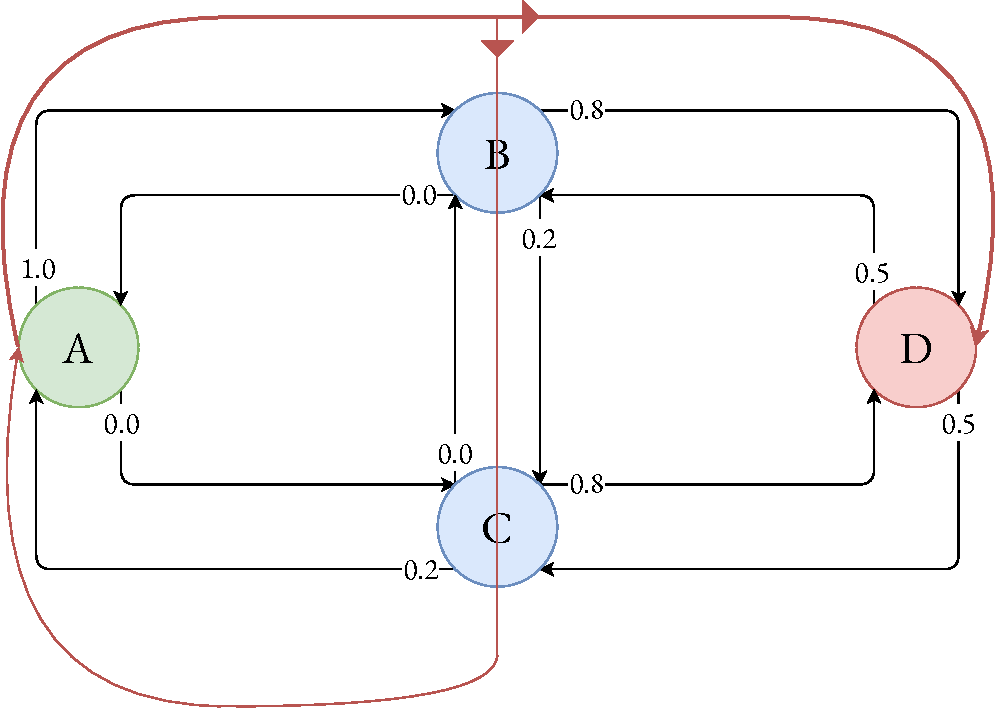
\includegraphics[width=0.8\textwidth]{figures/bad_route.pdf}
    \caption{An example of a bad routing created by the softmin routing strategy. A loop between nodes A, B, and C causes excess link utilisation and increased latency. The circles are vertices with A being the flow source and D the flow destination. The black lines are edges with the numbers signifying their splitting ratios. The red line is the flow induced by this particular routing.}
    \label{fig:bad_route}
\end{figure}


\todo{split pruning into separate section and writeup new alg}
\todo{cite DODAG and RLP and NP-hardness}
It can easily be seen that the problem of loops in the routing would not exist in a directed acyclic graph (DAG) as they are defined to have no cycles. Therefore, one way of avoiding routing loops is to convert the graph into a DAG by breaking links. A natural way to think about this is that for a path in a graph to be a cycle, it has to loop backwards on itself at some point. This means that at some point it is taking a step further away from the destination of the flow and back towards the source. As part of calculating the softmin routing we have already found the distance from each vertex to the destination. We can reuse this information to prune edges removing cycles. If, for every edge, we remove it if its head is further from the destination than its tail, then we know that traversing an edge can only ever bring us closer to the destination than we already are. If we remove all edges to more distant nodes then we have now created a DAG and so have no cycles. This method is also shown in algorithm~\ref{algorithm:softmin}.

\todo{write out the algorithm for softmin including pruning}
\begin{algorithm}[t]
\small
\begin{algorithmic}
\Function{GraphNetwork}{$E$, $V$, $\mathbf{u}$}
\EndFunction
\end{algorithmic}
\caption{Softmin routing algorithm: the steps taken to convert the learned edge weights given by the RL agent into a fully-defined routing strategy.}
\label{algorithm:softmin}
\end{algorithm}

\section{Traffic demand sequences}
We are using RL to approach this problem and the input to the agent is a history of previous demand matrices. The reason for this is that we have made the assumption that the sequence if DMs will have some sort of regularity which we can exploit to predict a routing strategy for the next timestep that is better than the optimal oblivious routing. Therefore, the demand sequences used for training such an agent must be built using some form of regularity. We try two different types of regularity heavily inspired by those selected by Valadrasky\cite{valadarsky2017learning}.

The first kind of regularity is \emph{cyclical}. Here we generate a cycle of demand matrices and the sequence is simply some number of repetitions of this cycle. The second kind is that of a \emph{gravity sequence}\cite{roughan2002experience}. This sequence again starts by defining a cycle which repeats but derives each subsequent DM as an averaging over the history rather than immediately presenting the next DM in the cycle. These scenarios make sense as temporal regularity is often seen in large networks such as those of ISPs\cite{fortz2002optimizing}. We also \emph{sparsify} the DMs (which consists of stochastically removing demands) to add noise to the regularity of the sequence.

\todo{Give mathematical definitions of DM sequences and sparsification}

The DMs in the cycles themselves are generated using a bimodal model\cite{medina2002traffic}. This is a model where demands are assigned randomly to flows, however, there is a small fixed probability that any such demand will be significantly larger than the rest (an elephant flow) which would impact the link utilisation if not handled carefully (thus aided by routing differently for different DMs).

\section{Training graphs}
For training and evaluation purposes it was important that the graphs trained on should be representative of real-world networks. It was thought that maybe graphs from this set could be generated. However, it is difficult to define the set of graphs akin to real-world AS networks. Fortunately, there is an open dataset, ``The Internet Topology Zoo''\cite{6027859} which contains a plethora of real-world networks, enough for both training and evaluation so it was decided to use this instead.


\chapter{Reinforcement learning methodology}
\todo[inline]{think of renaming this chapter to be less generic, more focussed on my project}

- the point of this chapter is to:
  - describe how the different policies have been designed (defo GNN, maybe LSTM, hopefully iter)
  - have some nice diagrams of the policy design maybe?
  - talk about modifications/translations of observation and action spaces to make them usable
  - talk about GNNs (encode -> process -> decode) and why (can vary obs + action size!)
  
 \section{Introduction}
 
- give a short into to why this chapter exists, what it seeks to do

\section{Environment interface}

- talk about the interface to the environment and how it needed modifying (i.e. gamma, squishing DMs etc)

\section{Standard policies}

- quick bit about the MLP and LSTM baselines
- mention the thinking behind them
- mention why they are not enough for generalisation

\section{GNN policy}

- first give summary paragraph
- then talk about how GNNs work
- then talk about encode process decode model
- then talk about how inputs are set and outputs derived

\section{Iterative GNN policy}
(may have to cut this section unfortunately depending on how everything goes)
- first give summary paragraph
- then mention placeto
- then talk about node/edge embedding
- then talk about more shit

\chapter{Evaluation}
\label{chapter:evaluation}

\subsection{Aims}
\todo[inline]{Give (and discuss) goals of what evaluation seeks to show (should map onto contributions given earlier). Talk about progressive randomisation and maybe include the definition table). summarise what experiments will be performed}
So far we have described the problem, approaches to a solution, and how to build different RL approaches that seek to solve it. The aim stated at the beginning of this work was to use RL to perform generalisable data-driven routing. Therefore, this evaluation seeks to assess:

\begin{enumerate}
\item Are the different policies able to learn to provide a near-optimal routing for a demand?
\item Are the policies able to generalise this technique to unseen sequences of the same type?
\item Do they still generalise to unseen sequences from a different distribution?
\item Are they able to generalise onto different graphs using sequences form the same and different distributions?
\item Are these routing schemes applicable to real-world scenarios?
\end{enumerate}

In the course of this chapter these questions will be answered by a sequence of experiments testing all of these stated aims.

\subsection{Experimental setup}
\todo[inline]{training set up. hyperparameter tuning. specifics of algorithm used. callbacck with reference to DM generation methodology earlier}


\subsection{Baselines}
\todo[inline]{just a callback to their earlier description with reference (mlp \& lstm). introduce raeke routing if use. also mention shortest path }


\subsection{Learning static routing}
\todo[inline]{talk about single sequence, single cycle}


\subsection{Learning cyclic routing}
\todo[inline]{talk about adding cycles and training on one / multiple sequences. still only test from training set though}


\subsection{Generalising to unseen sequences}
\todo[inline]{talk about changing just the dms, changing the cycle length, even changing dm type}


\subsection{Generalising to unseen graphs}
\todo[inline]{mention again why not comparing mlp here. mention why important (drop node/link etc, ref earlier). do drop/add node/link. do gen from same distribution. do out of distribution (will probably fail but is good to show)}

\subsection{Real world}
\todo[inline]{test on TOTEM/Abilene dataset}



\chapter{Conclusions and future work}
\label{chapter:conclusions}

\section{Conclusions}
In this work we have sought to provide a generalisable approach to data-driven using deep \ac{rl} with \acp{gnn}. This has consisted of providing a detailed specification of the problem and presenting an environment which can be used to experiment with different techniques to see how well they perform. We also took the approach introduced by Valadarsky et al. and modified it extensively so that it both worked to spread traffic across multipath routes and so that it could work with \acp{gnn}. In addition, we designed \ac{gnn} policy architectures that could be used in conjunction with this problem and more generally provided a connection between an \ac{rl} library and variable-sized graph network models.

After presenting previous work as well as our new additions we performed extensive experiments on the different policy architectures in different scenarios to assess how well they generalise to different demand matrices followed by different kinds of regularity in demand sequences before finally looking at generalisation to different network topologies. These experiments showed that all these policies can learn to efficiently route a demand matrix, in fact multiple. They also showed that \acp{gnn} are able to generalise learned routings. Unfortunately they showed that we were unable to make any of the policies learn to route demand matrices based on a history of previous demands beyond providing a good oblivious routing that did a good job of minimising the utility function (in this case maximum link utilisation).

Overall there has been the presentation of new techniques and a new library along with a mixture of successes and failures. Fortunately we can draw on these failures to inspire new work.


\section{Future work}
As previous work as suggested that the approaches taken in this paper can be successful, we feel it is important for these approaches to be explored further. On core part of the approach taken has been in designing a good way to reduce the size of the action space. An important part of this was in designing a mapping from edge weights to a routing strategy. We feel that an exploration of different techniques mapping edge weights or indeed any intermediate structure to a routing could provide interesting results. Furthermore, the way that demand information is input to the network could be greatly improved through numerous techniques and possibly hierarchical \ac{rl} would be an interesting area to explore here.

Beyond mappings of observations and outputs there are many different ways in which the learning itself could be modified. These include using different learning algorithms to \ac{ppo} and employing different techniques for graph generalisation such as the iterative approach. Another aspect that could be looked into here are modifications to the reward function with different properties that could aid exploration. Finally, we saw some successes with varied sequence length from the \ac{lstm} approach so if this could be combined with a method allowing for generalisation to different graphs it could lead to an approach achieving the best of both worlds.

Assuming the success of techniques presented here, this work can be expanded to explore optimisations of routing to perform different goals, such as in changing the utility function. A natural next step would be implementing these strategies in real-world \ac{sdn} systems so that that could be tested and used on real-world networks. This would present new challenges, mainly centred around managing incomplete information and distributing control.

We did see success with the generalisation ability of \acp{gnn} which suggests that outside of the area of data-driven routing there may be other useful application to explore. Other aspects of network control have been investigated with \ac{ml} and particularly RL techniques such as resource scheduling and rate controls which may benefit greatly from the application of \ac{gnn}-based techniques.



\appendix
\singlespacing

\printbibliography

\end{document}
